%%%%%%%%%%%%%%%%%%%%%%%%%%%%%%%%%%%%%%%%%%%%%%%%%%%%%%%%%%%%
%%%%%%%%%%%%%%%%%%%%%%%%%%%%%%%%%%%%%%%%%%%%%%%%%%%%%%%%%%%%
\subsection{Koordinatensysteme}
Kartesische Koordinaten, Polarkoordinaten, etc.

\mrnote{vorläufig sind die Folien aus Carl Herrmanns Teil zu Koordinatensystemen eingefügt. Die Beispiele beziehen sich noch auf Kapitel 2, da der Themenkomplex ursprünglich dort angesiedelt war}

\begin{frame}
    \frametitle{Koordinatensysteme}

    \begin{itemize}
        \item Es gibt unterschiedliche {\bf Koordinatensysteme}, um die Position eines Punktes im Raum zu beschreiben
        \item Beispiele:
        \begin{enumerate}
            \item Kartesische Koordinaten $(x,y,z,...)$
            \item Polarkoordinaten im 2d Raum: $(r,\theta)$
            \item Kugelkoordinaten im 3d Raum $(r,\theta,\phi)$
        \end{enumerate}
        \item Die Wahl des Koordinatensystems is beliebig, aber bestimmte Systeme eignen sich besser als andere, und führen zu einer einfachen Beschreibung.
    \end{itemize}
\end{frame}

%%%%%%%%%%%%%%%%%%%%%%%%%%%%%%%%%%%%%%%%%%%%%%%%%%%%%
\begin{frame}
    \frametitle{Polarkoordinaten}

\begin{center}
    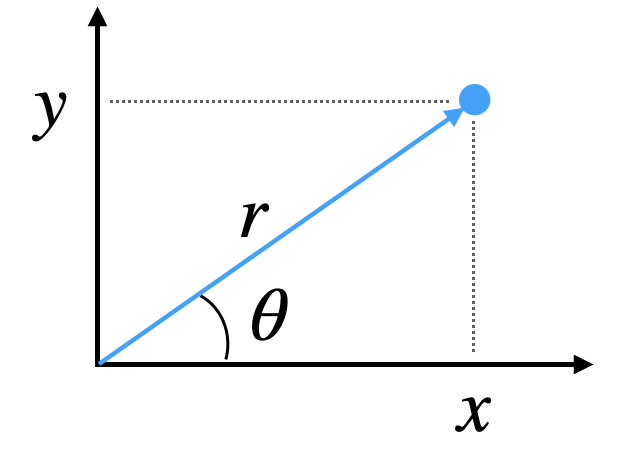
\includegraphics[width=.3\textwidth]{fig/pk11.png}
\end{center}


 \begin{itemize}
    \item im 2-dimensionalen Raum kann jeder Punkte entweder durch kartesische Koordinaten $(x,y)$ oder durch Polarkoordinaten $(r,\theta)$ beschrieben werden.
    \item Umwandlung von Polarkoordinaten in kartesische Koordinaten:
$$
\left\{\begin{array}{l} x = r\cos\theta \\ y = r\sin\theta \end{array}\right. ~~~\text{mit}~~r\ge 0, ~~~\theta \in [0,2\pi)~(\text{oder}~\theta \in [-\pi,\pi))
$$
     \item Umwandlung von kartesischen in Polarkoordinaten:
     $$
    \frac{y}{x} = \frac{r\sin\theta}{r\cos\theta} = \tan\theta~;~~~~r=\sqrt{x^2+y^2}
     $$
 \end{itemize}
\end{frame}

%%%%%%%%%%%%%%%%%%%%%%%%%%%%%%%%%%%%%%%%%%%%%%%%%%%%
\begin{frame}
    \frametitle{Polarkoordinaten}
    \begin{itemize}
     \item Achtung: da die Umkehrfunktion $\arctan$ definiert ist von $\mathbb{R}\rightarrow (-\frac{\pi}{2},\frac{\pi}{2})$ liefert diese Formel nur einen Winkel zwischen $-\frac{\pi}{2}$ und $\frac{\pi}{2}$!
     \item je nachdem, in welchem Quadranten sich der Punkt befindet, muss man den Winkel anpassen.
 \end{itemize}   
\begin{center}
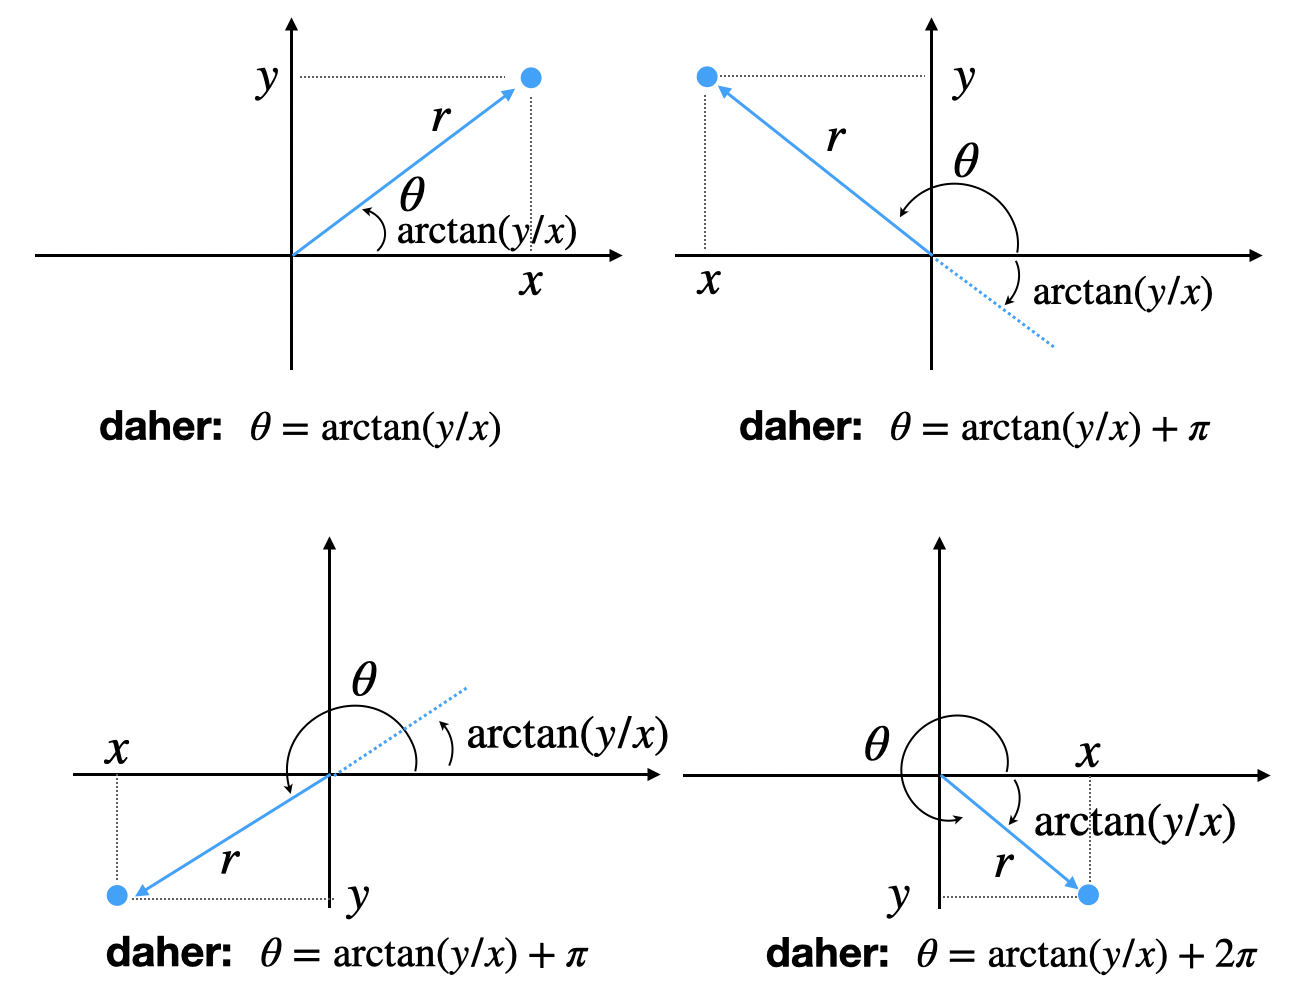
\includegraphics[width=.7\textwidth]{fig/pk13.png}
\end{center}
\end{frame}

%%%%%%%%%%%%%%%%%%%%%%%%%%%%%%%%%%%%%%%%%%%%%%%%%%%%
\begin{frame}
    \frametitle{Beispiele von Parametrisierungen}


    {\bf Kreis}, Mittelpunkt bei $(0,0)$, Radius $a$:
    \begin{columns}
        \begin{column}{0.7\textwidth}
        \begin{itemize}
            \item $\text{kartesische Koordinaten:}~\sqrt{x^2+y^2}=a$
            \item $\text{Polarkoordinaten:}~ r=a, ~\theta\in[0,2\pi)$
        \end{itemize}
    \end{column}
    \begin{column}{0.3\textwidth}
        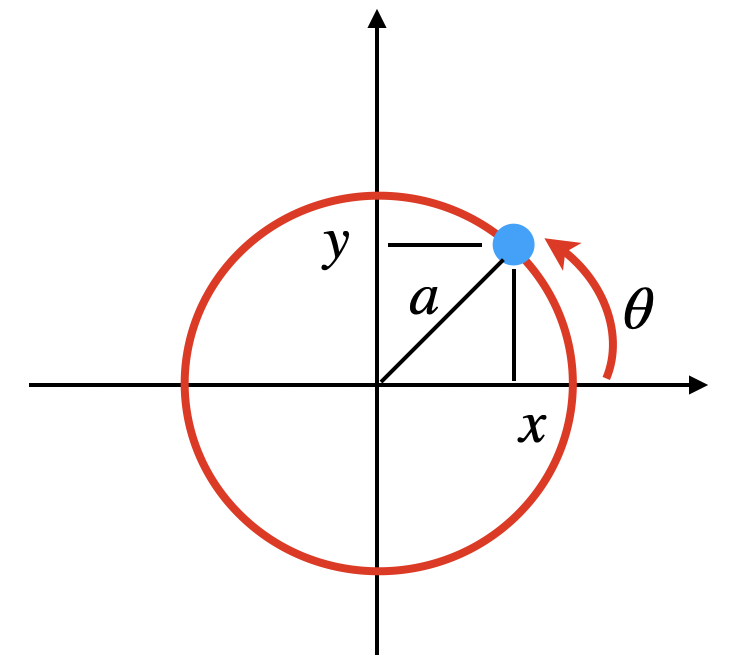
\includegraphics[width=\textwidth]{fig/pk14.png}
    \end{column}
\end{columns}
        {\bf Halbgerade:}
        \begin{columns}
            \begin{column}{0.75\textwidth}
        \begin{itemize}
            \item $\text{kartesische Koordinaten:}~y=ax$ mit $x,y,a>0$
            \item $\text{Polarkoordinaten:}~ \theta=\text{Konstante mit}~~ \cos\theta = \frac{1}{\sqrt{1+a^2}}~, r\ge 0$
        \end{itemize}
    \end{column}
    \begin{column}{.25\textwidth}
        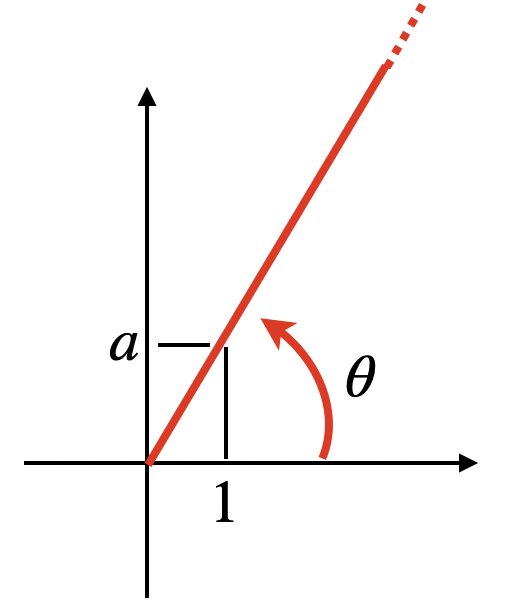
\includegraphics[width=\textwidth]{fig/pk15.png}
    \end{column}
\end{columns}
    

\end{frame}



%%%%%%%%%%%%%%%%%%%%%%%%%%%%%%%%%%%%%%%%%%%%%%%%%%%%
\begin{frame}
    \frametitle{3D: Kugelkoordinaten}

    \begin{columns}
        \begin{column}{.6\textwidth}
    \begin{itemize}
        \item Verallgemeinerung der Polarkoordinaten in 3d
        \item $(x,y,z)~\longrightarrow~(r,\theta,\phi)$
        \item $r$ = Radius $(r\ge 0)$
        \item $\theta$ = Polarwinkel $(0\le \theta\le \pi)$
        \item $\phi$ = Azimutwinkel $(0\le \phi\le 2\pi)$
    \end{itemize}
\end{column}
\begin{column}{.4\textwidth}
    \begin{center}
        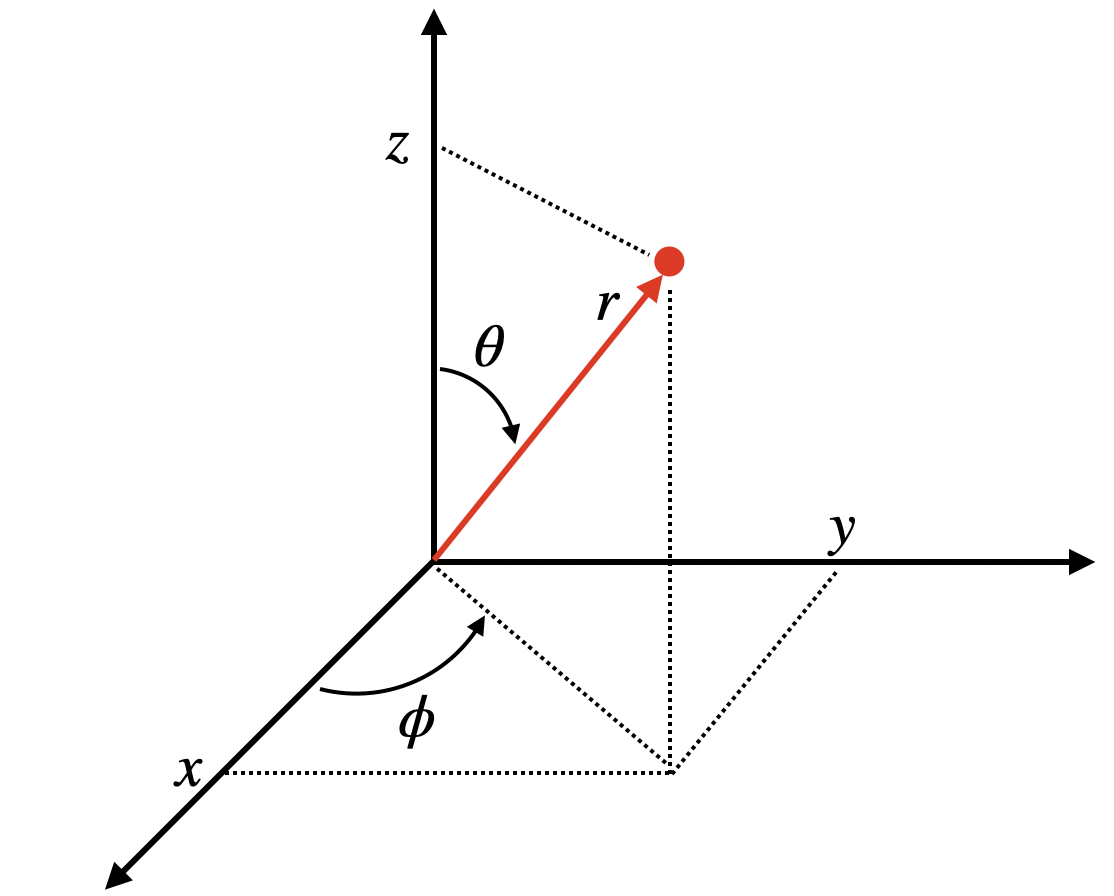
\includegraphics[width=\textwidth]{fig/pk18.png}
    \end{center}
\end{column}
\end{columns}
\vspace{.5cm}
Kugelkoordinaten $\longrightarrow$ kartesische Koordinaten:
\begin{itemize}
    \item $x = r\,\sin\theta\,\cos\phi$
    \item $y=r\,\sin\theta\,\sin\phi$
    \item $z=r\,\cos\theta$
\end{itemize}

\end{frame}



%%%%%%%%%%%%%%%%%%%%%%%%%%%%%%%%%%%%%%%%%%%%%%%%%%%%
\begin{frame}
  \frametitle{Parametrische Kurven in verschiedenen Koordinatensystemen}
  
  \begin{itemize}
  \item Wenn wir die Bewegung eines Punktes im 2d/3d Raum beschreiben, können wir die {\bf zurückgelegte Strecke} $L$ oder die {\bf überstrichene Fläche} $S$  bestimmen.
  \item Dazu muss ein infinitesimales Streckenstück $dL$ oder Flächestück $dS$ integriert werden.
  \item Der Ausdruck von $dL$ oder $dS$ hängt vom {\bf Koordinatensystem} ab!
  \end{itemize}
  \begin{center}
    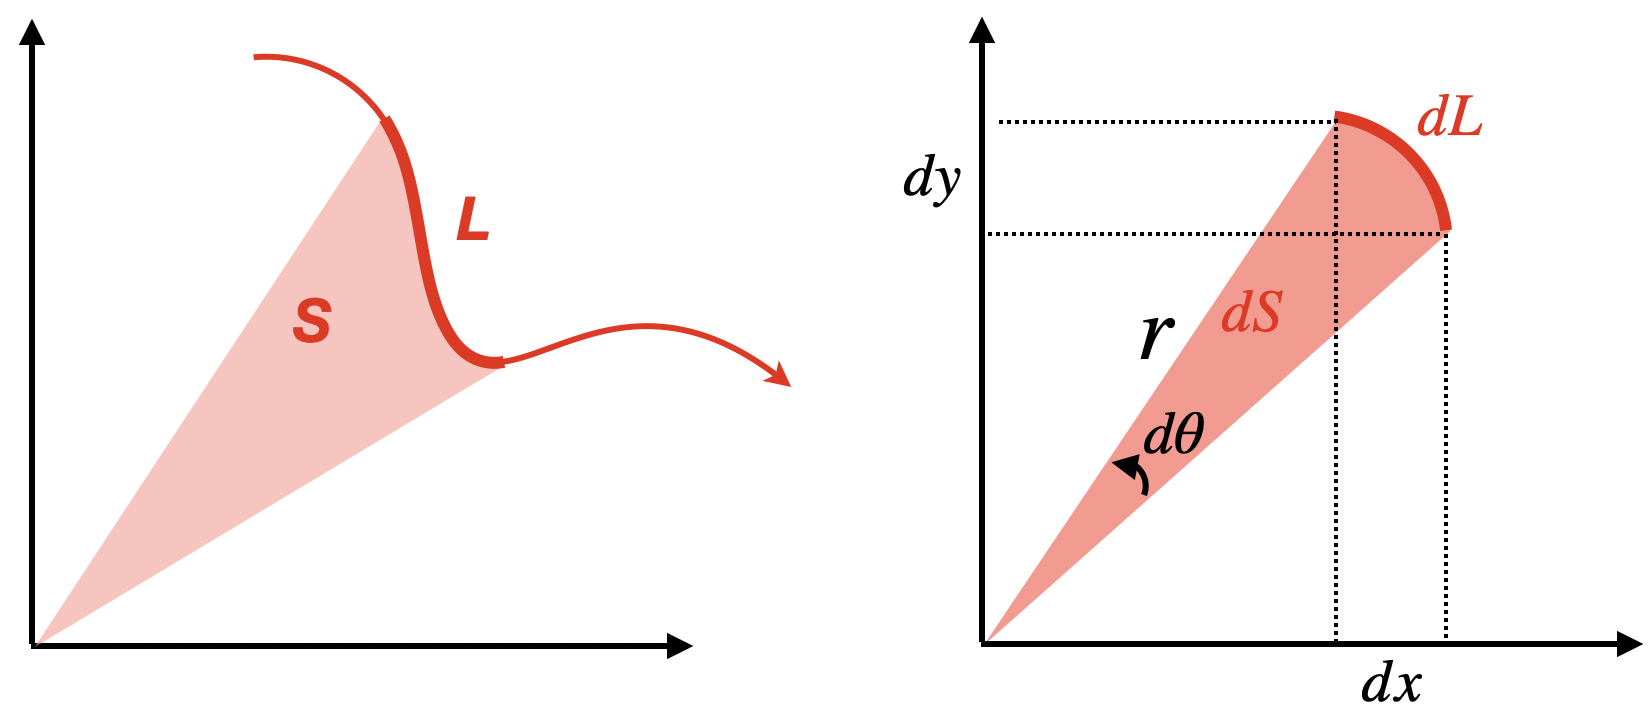
\includegraphics[width=.8\textwidth]{fig/pk21.png}
  \end{center}
\end{frame}

